%%%%%%%%%-----------------------------------------------------------------
%%%%%%%%% Thesis template, v1
%%%%%%%%% Mathematical & Statistical Methods group - Biometris
%%%%%%%%% Wageningen University & Research
%%%%%%%%%-----------------------------------------------------------------


\documentclass{amsart}

\usepackage{booktabs}
\usepackage{lipsum}

% Setting margins
\usepackage[a4paper, left=3cm,right=3cm]{geometry}

% Packages for the titlepage
\usepackage{tikz}
\usetikzlibrary{calc}
\usepackage{graphicx}
\usepackage{newtxtext}
\usepackage{float}

% Packages for mathematical writing
\usepackage{amsmath}                           % Enables the align enviroment
\usepackage{amssymb}                           % Math symbols (e.g. \mathbb{})
\usepackage{dsfont} 	                         % For \mathds{1} blackboard bold 1
\usepackage{bm}                                % For roman (upright) bold latin letters
\usepackage{mathtools}                         % Better math
\usepackage[hypertexnames=false]{hyperref}     % For urls and hyperlinks
\usepackage[scientific-notation=true]{siunitx} % For scientific notation

% For theorems, remarks, lemmas etc.
\usepackage{amsthm}
\theoremstyle{plain}
\newtheorem{theorem}{Theorem}%[section]
%% >> Define your newtheorems here

% For algorithms
\usepackage[ruled,vlined]{algorithm2e}
\usepackage{algpseudocode}
\renewcommand{\algorithmicrequire}{\textbf{Input:}}
\renewcommand{\algorithmicensure}{\textbf{Output:}}

% Often used math operators:
% You can define these yourself using \DeclareMathOperator and \newcommand
%\DeclareMathOperator*{\argmax}{arg\,max}    % maxmizing argument
%\newcommand{\LA}{\mathbf{\Lambda}}

% For bibliography
\usepackage[numbers]{natbib}
\def\bibfont{\footnotesize}


%--------------------------------------------------------------------
%--------------- Front and Main matter style ------------------------
\newcommand{\frontmatter}{
    \pagenumbering{roman}   % Setting page numbering to lower-case roman
}
\newcommand{\mainmatter}{
    \newpage
    \pagenumbering{arabic}  % Setting page numbering to normal integers
}
%--------------- Front and Main matter style ------------------------
%--------------------------------------------------------------------

\usepackage{Sweave}
\begin{document}
\Sconcordance{concordance:Thesis_Template_Biometris.tex:Thesis_Template_Biometris.rnw:1 %
65 1 1 0 345 1 1 9 11 0 1 2 136 1}



% Add title page:
%------------------------------------------------------------------------------
% In this segment, enter the desired student data to be shown at the title page
\newcommand{\thesisAuthor}{George Miliarakis}                             % State your name
\newcommand{\thesisTitle}{Predicting APOE-4 status with plasma metabolomics panel in Alzheimer's Disease}                                      % State title thesis
\newcommand{\thesisSubTitle}{A Machine Learning approach}                            % State subtitle thesis
\newcommand{\thesisDegree}{Master thesis project}      % Choose type
\newcommand{\university}{Wageningen University \& Research}                % You generally don't need to touch this
\newcommand{\thesisPlaceDate}{Wageningen, Month Year}                      % State month and year
%------------------------------------------------------------------------------


%------------------------------------------------------------------------------
% In this segment, enter the desired supervisor data to be shown at the title page
\newcommand{\supervisor}{C.F.W. Peeters}                                                % State name of supervisor
\newcommand{\departmentSUP}{Mathematical \& Statistical Methods group (Biometris)} % State department supervisor (generally Biometris)
\newcommand{\universitySUP}{Wageningen University \& Research}                              % State university supervisor (generally WUR)
%------------------------------------------------------------------------------


%------------------------------------------------------------------------------
% In this segment, enter the desired co-supervisor data to be shown at the title page
\newcommand{\cosupervisor}{Yannick Vermeiren}                                         % State name of co-supervisor
\newcommand{\departmentCOSUP}{Nutrition, Brain and Cognitive Ageing}                             % State department or division co-supervisor
\newcommand{\universityCOSUP}{Wageningen University \& Research}                              % State university or company co-supervisor
%------------------------------------------------------------------------------


%------------------------------------------------------------------------------
% Logos and visuals
\begin{titlepage}
\thispagestyle{empty}

% Adding logos
\begin{figure} [H]
\vspace{-3cm}
 \centering
\begin{minipage}[t]{.45\linewidth}
  \raggedright
  % Upload and include SLU loggo here:
  \hspace*{-2cm}
\includegraphics[width=\linewidth]{~/figures/WURlogo.png}

\end{minipage}%
  \begin{minipage}[t]{.45\linewidth}
  \vspace{-2.6cm}
 \raggedleft
%% Inclusion Biometris logo
 \hspace*{+2cm}
\includegraphics[width =.95\textwidth]{figures/biometris_logo.png}

\end{minipage}
\end{figure}

% Bottom/background picture
\begin{tikzpicture}[overlay, remember picture]
\node[anchor=south west,
      xshift=+6.5cm,
      yshift=-0.2cm]
     at (current page.south west)
     {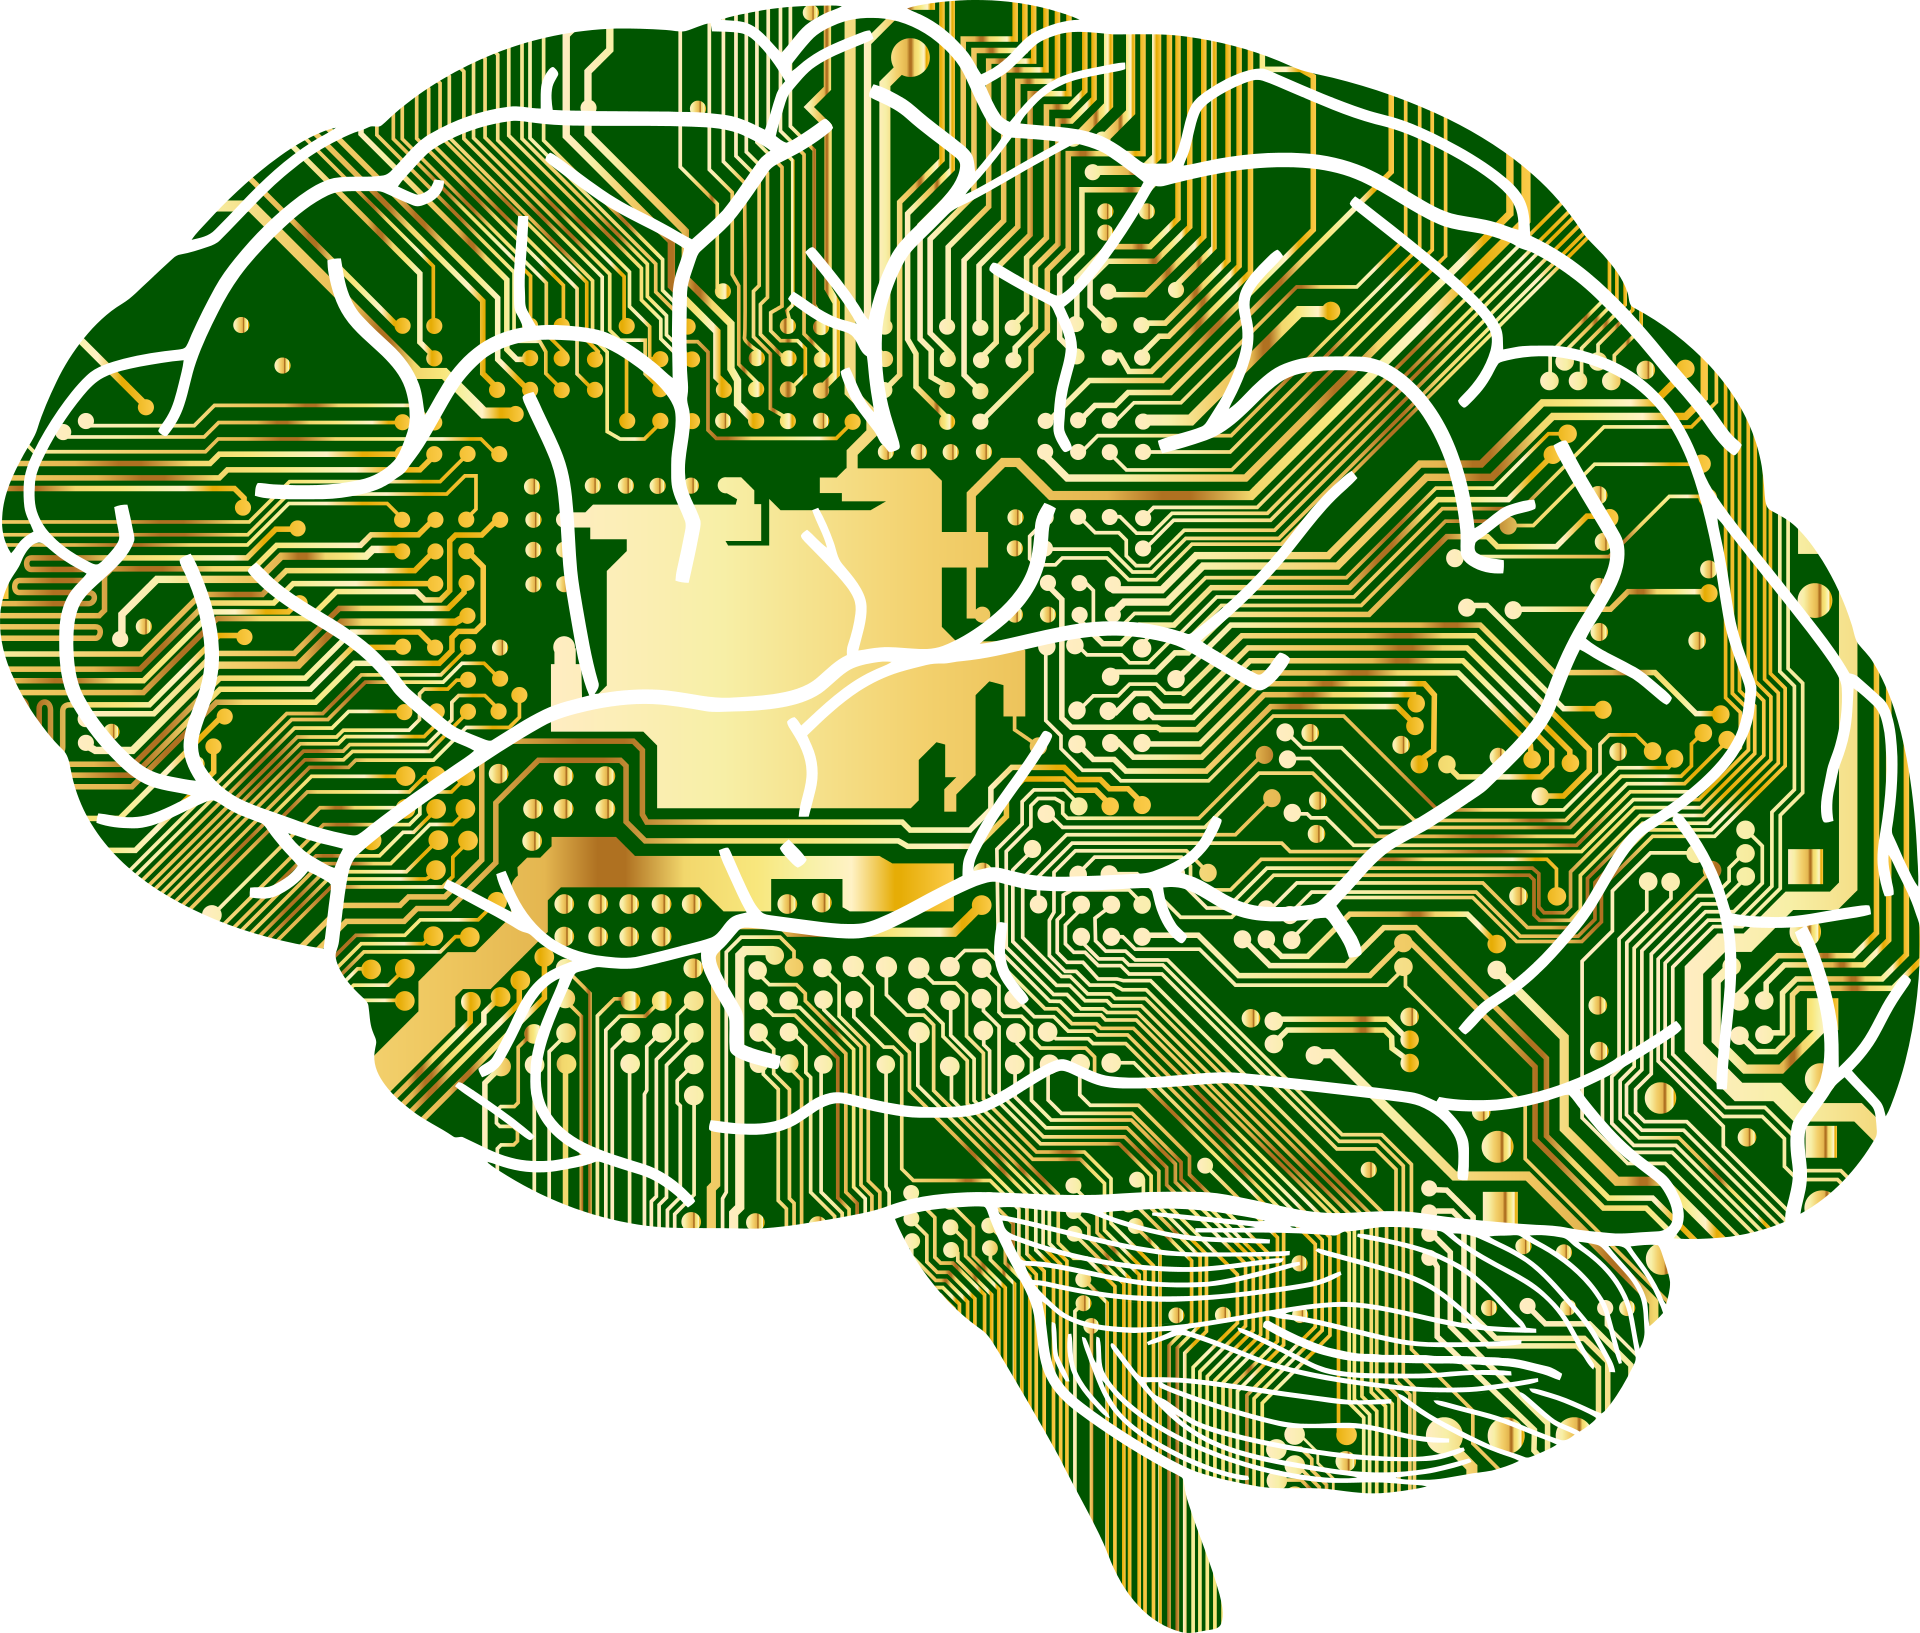
\includegraphics[width = .5\textwidth]{figures/green_brain.PNG}};
\end{tikzpicture}
%------------------------------------------------------------------------------


%------------------------------------------------------------------------------
% Title information
\vspace{1cm}
\begin{center}
\par
\noindent
\rule[0.2cm]{\linewidth}{1.5pt}
\Huge
\textbf{\thesisTitle}
\vspace{0.2cm}
\LARGE
\par
\noindent
\thesisSubTitle\\
\rule[0.2cm]{\linewidth}{1.5pt}
\Large
\end{center}
%------------------------------------------------------------------------------


%------------------------------------------------------------------------------
% Author information
\vspace{2cm}
\noindent
\LARGE
\thesisAuthor\\
\vspace{.2 cm}
\small
\par \noindent
\thesisDegree
\par \noindent
\university
\par \noindent
\thesisPlaceDate
%------------------------------------------------------------------------------


%------------------------------------------------------------------------------
% Supervision information
\vspace{4cm}
\begin{flushright}
\emph{Supervisor} \\
\textbf{\supervisor} \\
\departmentSUP \\
\universitySUP
\end{flushright}

\vspace{.5cm}
\begin{flushright}
\emph{Co-supervisor} \\
\textbf{\cosupervisor} \\
\departmentCOSUP \\
\universityCOSUP
\end{flushright}
%------------------------------------------------------------------------------


\end{titlepage}


% Spacing pages
\clearpage\thispagestyle{empty}
\newpage
\mbox{}
\clearpage
\newpage
\frontmatter


% Foreword
\section*{Foreword}
This is where you type your foreword.
In the Foreword the student states clearly his/her contribution that originates from the master thesis project, and, if applicable, what contribution(s) possibly followed from the students' internship on the same topic.
It is also stated in the foreword what data sources were used, and whether the data have a degree of confidentiality.
In addition, possible acknowledgements may be made to people who have contributed to (certain parts of) the thesis.


% Abstract
\newpage
\section*{Abstract}
This is where you type your abstract.
The abstract must be communicable to a broad audience and contain, next to a summary text, an outreach item such as an infographic or a link to a video/website/web application.
Such as, for example, the nice figure below.
\begin{figure}[h!]
\centering
  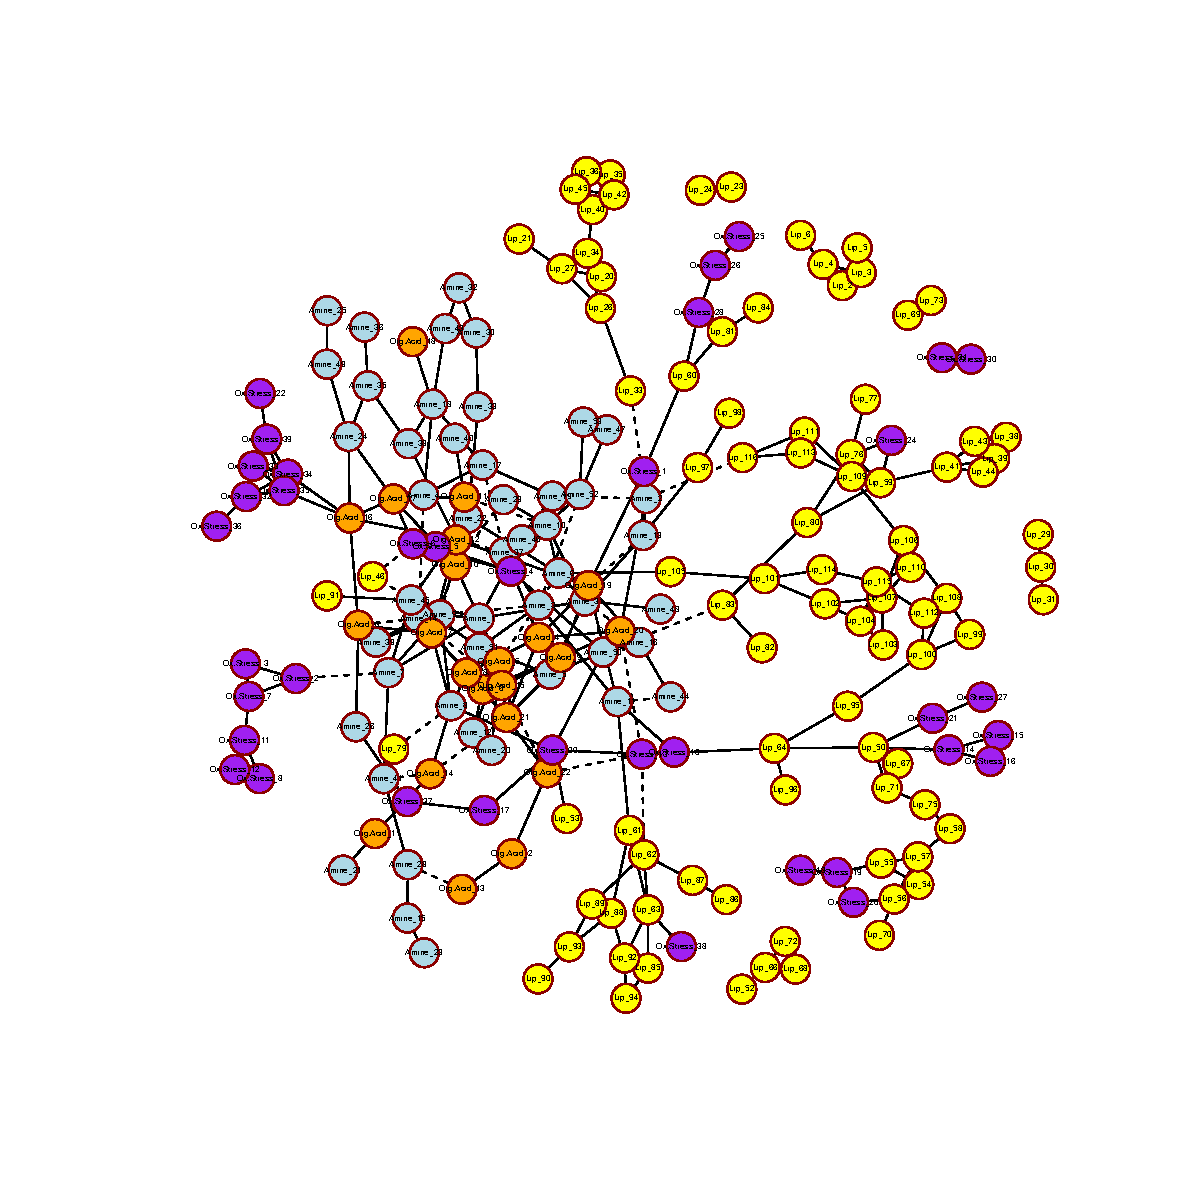
\includegraphics[width=\textwidth]{figures/NTWK.pdf}
    \caption{A nice figure}
  \label{FIG:NTWK2}
\end{figure}



% Inserting table of contents
\newpage
\tableofcontents
%--------------- Front matter ---------------------------------------
%--------------------------------------------------------------------






%--------------------------------------------------------------------
%--------------- Main matter ----------------------------------------
\cleardoublepage
\mainmatter

\section{Introduction}\label{Intro}
Welcome to the Biometris \texttt{Rnw} thesis template.
\textsf{R} includes a flexible system (\textsf{knitr}) for creating reproducible dynamic reports using \LaTeX. 
It enables you to embed \textsf{R} code within \LaTeX \, documents which can be compiled from within your \texttt{RStudio} environment.
\LaTeX is a high-quality typesetting system designed for technical and scientific documentation.
It is available through free distribution systems as \href{https://miktex.org/}{MikTex}.
This document simultaneously provides a quick introduction to running \LaTeX \, through \texttt{RStudio} and an overview of the structure of a Biometris thesis.
More information on \textsf{knitr} can be found \href{https://support.rstudio.com/hc/en-us/articles/200552056-Using-Sweave-and-knitr}{here}.


\subsection{The template}\label{Template}
\begin{sloppypar}
The main thesis template is contained in \texttt{Thesis\_Template\_Biometris.rnw}.
We recommend you rename this file to \texttt{YOURNAME\_ThesisBiometris.rnw}.
Upon compilation the \texttt{YOURNAME\_ThesisBiometris.PDF} will then be produced.
You might need to compile multiple times to produce your final PDF.
For compilation you will need \href{https://www.rstudio.com/}{RStudio}, \textsf{R}, its \textsf{knitr} package (and dependencies), as well as a \LaTeX \,distribution. 
\end{sloppypar}

The titlepage is contained within the main template.
You need to adapt the requested information (regarding, e.g., names and departments).
The titlepage is called from within the main template.

Front matter, main matter, and back matter are indicated within the main template.
Figures are contained in the folder called \emph{figures}.
Your text can be typed directly in the main template.


\subsection{Sectioning}\label{Subsec}
Sections are specified by \verb|\section{}|.
The name of your section can be specified between brackets.
Subsections are specified by \verb|\subsection{}|.
To cross-reference a section or subsection within your text you can mark your (sub)section with \verb|\label{}| and call the specified label with \verb|\ref| at the desired place.
Next to (sub)sections, you can also cross-reference equations, figures, tables, listings, etc.
As an example, let's reference Section 1 which has gotten the label \verb|\label{Intro}| by calling \verb|\ref{Intro}|, producing the following cross-reference link: \ref{Intro}.


\subsection{Equations}\label{Equations}
Your document may contain some equations.
Inline equations are produced by calling \verb|$$| and typing your mathematical symbols in between the dollar signs.
For example, \verb|$e^{i\pi} + 1 = 0$| will produce: $e^{i\pi} + 1 = 0$.
You might want to state important equations in display mode.
This can be done using the \LaTeX \,equation environment.
For example, we might call the following statement:
\begin{verbatim}
\begin{equation}\label{eq:Euler}
    e^{i\pi} + 1 = 0.
\end{equation}
\end{verbatim}
Wich will produce:
\begin{equation}\label{eq:Euler}
    e^{i\pi} + 1 = 0.
\end{equation}
As the equation has a label is can be cross-referenced.
Calling \verb|(\ref{eq:Euler})| will produce (\ref{eq:Euler}).
Equations are automatically and consecutively numbered.
In general it is considered good practice to only number equations to which you make an inline reference.
If you would like for an equation to be unnumbered, you can call the equation environment with the inclusion of an asterisk.
For example, calling
\begin{verbatim}
\begin{equation*}
    e^{i\pi} + 1 = 0.
\end{equation*}
\end{verbatim}
will produce the unnumbered equation:
\begin{equation*}
    e^{i\pi} + 1 = 0.
\end{equation*}

More information on mathematical expressions in \LaTeX \,can be found on \href{https://www.overleaf.com/learn/latex/mathematical_expressions}{Overleaf}.
A mathematical symbols cheat sheet can be found \href{https://www.caam.rice.edu/~heinken/latex/symbols.pdf}{here}.


\subsection{Figures}\label{Figures}
The template includes the \textsf{graphicx} package for handling figures.
The preferred extension is PDF.
An example of how to call a figure is as follows:
\begin{verbatim}
\begin{figure}[b!]
\centering
  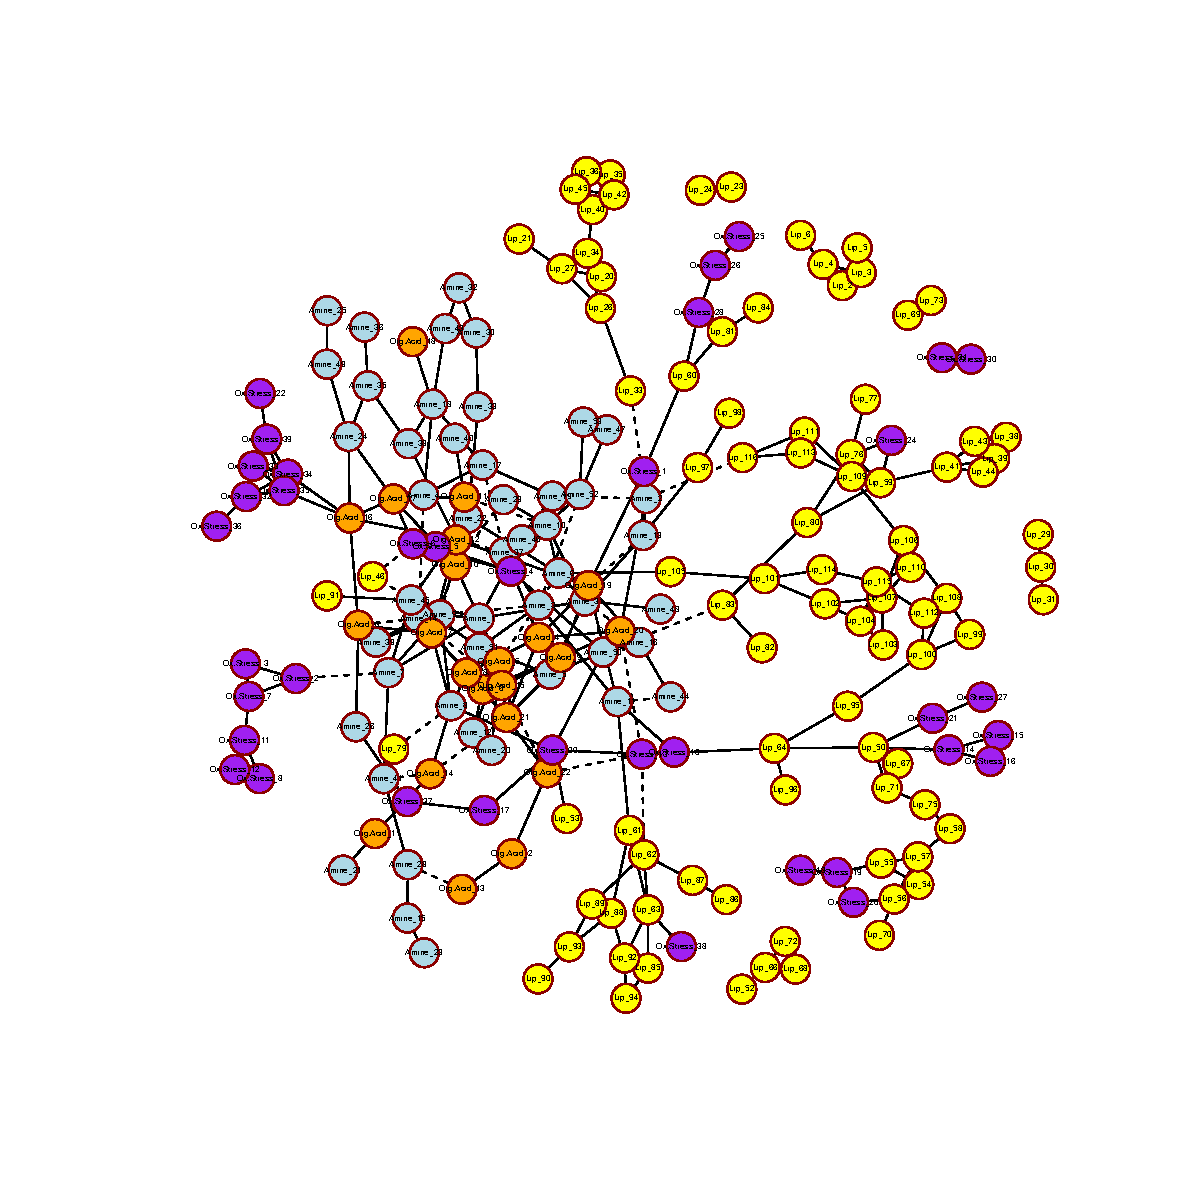
\includegraphics[width=.88\textwidth]{figures/NTWK.pdf}
    \caption{Your caption can contain any description of your figure.
    It can also contain math symbols: $\beta$.}
  \label{FIG:NTWK}
\end{figure}
\end{verbatim}
In this example the figures folder contains a figure called \verb|NTWK|.
We want to include this figure at the bottom of the page (\verb|[b!]|) at a width of $.88$ times the textwidth.
The figure gets the attached label \verb|FIG:NTWK|.
Calling this statement then produces the figure at the bottom of the page.
\begin{figure}[b!]
\centering
  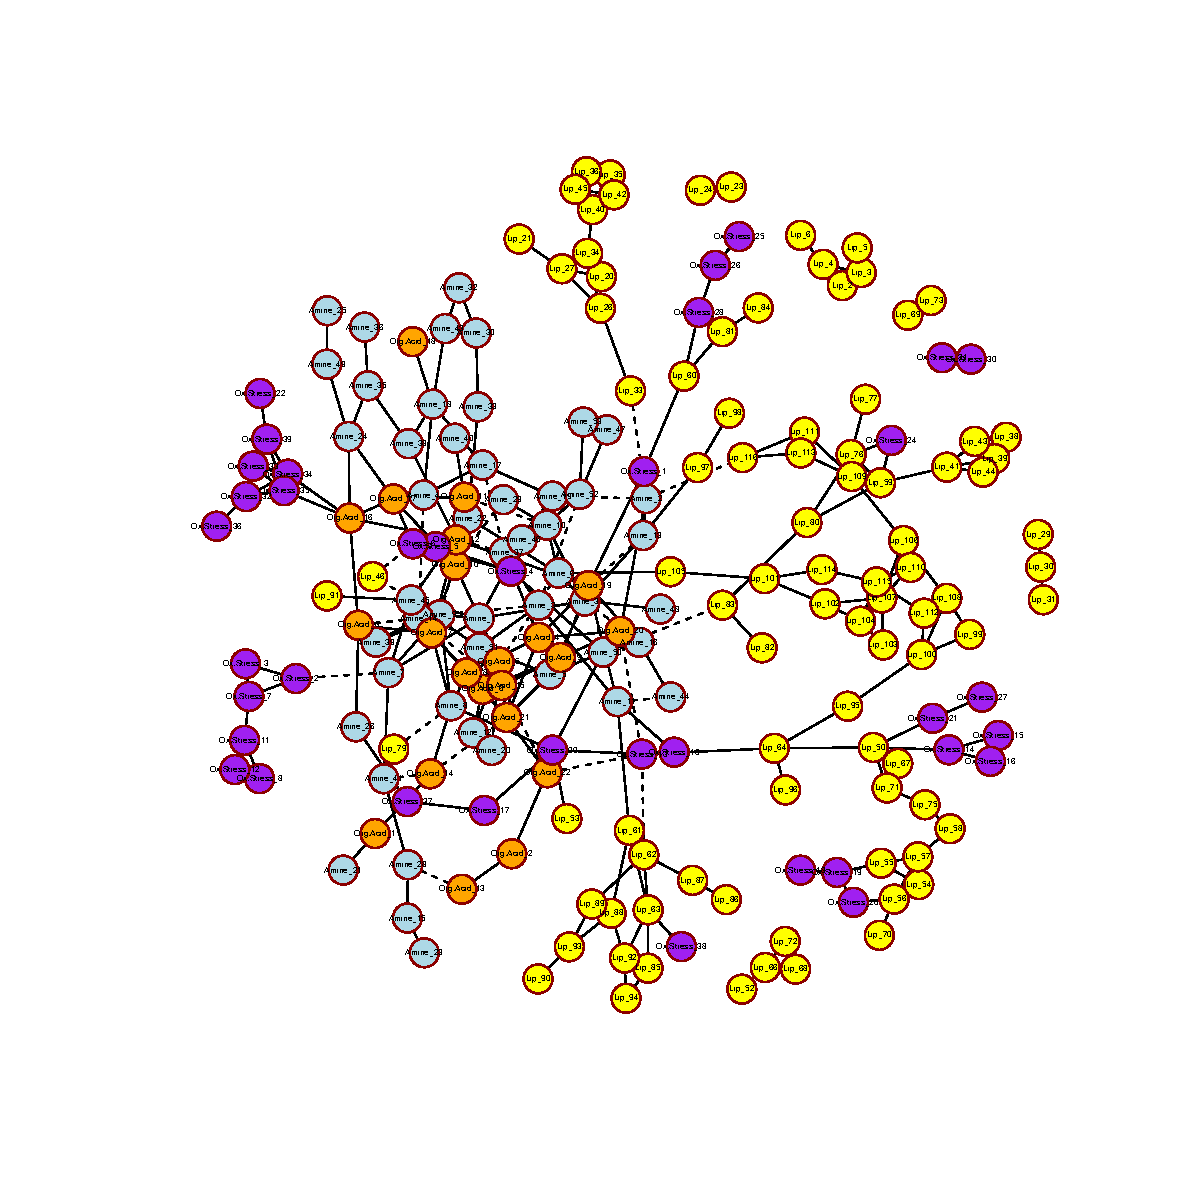
\includegraphics[width=.88\textwidth]{figures/NTWK.pdf}
    \caption{Your caption can contain any description of your figure.
    It can also contain math symbols: $\beta$.}
  \label{FIG:NTWK}
\end{figure}
The figure can be cross-referenced by referencing its label as \verb|\ref{FIG:NTWK}|: \ref{FIG:NTWK}.


\subsection{Tables}\label{Tables}
Your thesis will likely contain some tables.
\LaTeX \,has a large set of tools for generating customized tables.
Most of them use the \texttt{tabular} environment.
A simple call would be:
\begin{verbatim}
\begin{table}[h!]
\begin{tabular}{lcc} \hline
Something interesting & $\lambda$ & $\gamma$ \\ \hline
A  & $2$ & $3$ \\
B  & $4$ & $1$  \\ \hline
\end{tabular}
\caption{This is a caption to a table}
\label{Table:ex}
\end{table}
\end{verbatim}
In this example we have 3 columns with the first outlined left and the remaining columns centered: \verb|{lcc}|.
The \verb|\hline| statement inserts a horizontal line.
Each \verb|&| separates a cell and the double-backslash \verb|\\| sets the end of a row.
We want to include the table close to the text which calls it (\verb|[h!]|).
As the table has a label it can be cross-referenced in a fashion analogous to the examples given above.
Calling these lines then produces the following table:
\begin{table}[h!]
\caption{This is a caption to a table}
\begin{tabular}{lcc} \hline
Something interesting & $\lambda$ & $\gamma$ \\ \hline
Object A  & $2$ & $3$ \\
Object B  & $4$ & $1$  \\ \hline
\end{tabular}
\label{Table:ex}
\end{table}

More information on generating tables in \LaTeX \, can be found on \href{https://www.overleaf.com/learn/latex/tables}{Overleaf}.
For elaborate tables you can use the support offered by online \LaTeX \,table generators.
Such as the one offered \href{https://www.tablesgenerator.com/}{here}.


\subsection{Algorithms}\label{Algos}
Sometimes, you may want to include a description of an algorithm in your thesis.
This may be done by calling the \texttt{algorithm} environment.
Algorithms may contain equation and cross-references.
An example of how to produce Algorithm \ref{Algo1} below can be found in the \texttt{.tex} template.
More information on generating algorithms in \LaTeX \, can be found on \href{https://www.overleaf.com/learn/latex/algorithms}{Overleaf}.

\begin{algorithm}[H]\label{Algo1}
\SetAlgoLined
\algorithmicrequire ~Something great \\
\algorithmicensure ~Something even greater \\
 initialization\;
 \While{While condition}{
  instructions\;
  \eIf{condition}{
   instructions1\;
   instructions2\;
   }{
   instructions3\;
  }
 }
 \caption{How to write algorithms}
\end{algorithm}


\subsection{Code listings}\label{Codes}
All tables and figures so far have been produced with \LaTeX \, statements.
It is also possible to produce them through R code embedded in your \texttt{rnw} document.
This way you can integrate your analysis (in \textsf{R}) with your writing.
It is possible to (selectively) include parts of your code when this aids (the readability of) your thesis.
This may all be done by using code chunks in your document.
Below you can find an echoed code chunk (meaning a chunk of code that is reproduced in the compiled document).
How to specify such a chunk can be found in the \texttt{.rnw} template file.

\begin{Schunk}
\begin{Sinput}
> ## Produce the graph
> Ugraph(PcorP,
+        type = "fancy",
+        lay = "layout_with_fr",
+        Vcolor = Colors,
+        prune = TRUE,
+        Vsize = 7,
+        Vcex = .3)
\end{Sinput}
\end{Schunk}

More information on (formatting of) code chunks and how to integrate them into your report can be found \href{https://www.chairejeanmorlet.com/uploads/1/5/4/5/15454822/stoehr.pdf}{here}.


\subsection{Special mathematical environments}\label{Maths}
In some cases you might need mathematical environments because you want to state a theorem/proposition and its proof.
The template uses the \texttt{amsthm} package for this purpose.
A theorem and proof environment are predefined.
You may define all kinds of additional special formatting environments.
Information on how to do so can be found \href{https://www.overleaf.com/learn/latex/theorems_and_proofs}{here}.

Below you will find an example of a theorem and proof statement.
How to specify these statements can be found in the \texttt{.tex} template file.

\begin{theorem}\label{ExampleTheorem}
If $m \in \mathbb{Z}$ is even, then $m^2$ is even.
\end{theorem}

\begin{proof}
Suppose $m \in \mathbb{Z}$ is even.
By definition, there exists an $n \in \mathbb{Z}$ such that:
\begin{equation*}
m = 2n.
\end{equation*}
Then we have
\begin{equation*}
m^2 = (2n)^2 = 4n^2 = 2(2n^2),
\end{equation*}
implying that $m^2$ is also even.
\end{proof}


\subsection{Referencing}\label{REFS}
The \texttt{natbib} package is used for referencing.
The easiest way is to add references in an embedded manner.
References are then added to the reference list by adding \verb|bibitems| to the \verb|thebibliography| environment (see the .tex file).
By manually specifying your \verb|bibitems| you can make your references comply with standard citation styles such as \href{https://en.wikipedia.org/wiki/Citation}{APA, Chicago, or Harvard}.
There are two basic citation commands: \verb|\citet| and \verb|\citep|.
The first is textual, the second parenthetical.
The second is the most appropriate command for embedded bibliographies.

As an example, consider the bibliography of this template:
\begin{verbatim}
\begin{thebibliography}{10}
\bibitem{Musings} Doe, J. \& Baloney, P. (2021).
Musings on the flying Spaghetti Monster.
\emph{Journal of Abnormal Findings}, 4:3--43.

\bibitem{Important} Schnitzel, W. (2020).
Undoubtedly important thoughts.
\emph{Journal of Important Thoughts}, 24:90-110.
\end{thebibliography}
\end{verbatim}
It has two entries, one labelled as \verb|{Musings}|, the other labelled as \verb|{Important}|.
Calling \verb|\citep{Musings}| will produce: \citep{Musings}.
You can make multiple citations by including multiple citation keys/labels in the \verb|\citep| call.
For example, calling \verb|\citep{Musings,Important}| will produce: \citep{Musings,Important}.

One could alternatively use \texttt{BibTex}: a bibliography management tool for \LaTeX.
When you use \texttt{BibTex} the entries for the bibliography are kept in a separate file which is to be imported into the main template.
Usage of \texttt{BibTex} gices more flexibility in handling citations than the embedded approach.
More information on using \texttt{BibTex} can be found \href{https://www.overleaf.com/learn/latex/Bibliography_management_with_bibtex}{here}.





\newpage
\section{Methods}
This is where you put the main body of your work.
You may change the section title when appropriate.
You may also use subsections as deemed appropriate.
Make sure that each Figure, Table, Algorithm, and Listing is provided with a self-explanatory caption.
In case you do not want this section to begin on a separate page then remove \verb|\newpage| before the \verb|\section| statement.



\newpage
\section{Results}
This is where you discuss your results.
You may change the section title when appropriate.
You may also use subsections as deemed appropriate.
Make sure that each Figure, Table, Algorithm, and Listing is provided with a self-explanatory caption.
In case you do not want this section to begin on a separate page then remove \verb|\newpage| before the \verb|\section| statement.



\newpage
\section{Discussion}
This is where you critically discuss what you have done and where you relate it to other work.
Again, if you don't want this section to begin on a separate page then remove \verb|\newpage| before the \verb|\section| statement.
%--------------- Main matter ----------------------------------------
%--------------------------------------------------------------------




%--------------------------------------------------------------------
%--------------- References -----------------------------------------
\newpage
\begin{thebibliography}{10}
\bibitem{Musings} Doe, J. \& Baloney, P. (2021).
Musings on the flying Spaghetti Monster.
\emph{Journal of Abnormal Findings}, 4:3--43.

\bibitem{Important} Schnitzel, W. (2020).
Undoubtedly important thoughts.
\emph{Journal of Important Thoughts}, 24:90-110.
\end{thebibliography}
%--------------- References -----------------------------------------
%--------------------------------------------------------------------




%--------------------------------------------------------------------
%--------------- Back matter ----------------------------------------
\newpage
\appendix
\section{Name of first appendix}
Your thesis might also contain appendices containing material in support of the Main Text.
The backmatter portion of the thesis template contains the \verb|\appendix| statement.
Each section that you specify (see Section \ref{Subsec}) after this statement will be considered an Appendix.


\section{Name of second appendix}
You can specify as many appendices as you like.
%--------------- Back matter ----------------------------------------
%--------------------------------------------------------------------



\end{document}



% This is a template for a thesis at Biometris created by C.F.W. Peeters in 2021 
